%---------------------------------------------------------------------------%
%->> Section 3.1: 问题分析
%---------------------------------------------------------------------------%

\section{问题分析}

前文已经指出，现有大模型智能体驱动的根因定位方法在故障表征、经验沉淀和在线执行稳定性方面仍存在不足。本章进一步回答一个更具体的问题：如何让大语言模型智能体在诊断经验知识的指导下完成根因定位，并在诊断过程中持续积累和更新相关经验知识。具体包括以下三个方面：

\begin{enumerate}[label=（\arabic*）]
    \item \textbf{有效的故障可观测数据统一表示与特征提取方法。}微服务系统中的指标、日志和调用链路在数据结构、时间粒度和语义层级上存在明显差异。若不能将这些观测转化为统一、稳定且可比较的故障表示，历史故障便难以用于当前场景的检索与匹配。

    \item \textbf{基于有效诊断自动构建 SOP 知识的方法。}运维经验分散在历史工单、排查记录和人工操作过程中，其中虽然包含大量判断依据和路径选择信息，但缺乏统一结构，既难以被智能体直接调用，也难以随着新故障的出现持续更新。

    \item \textbf{兼顾探索深度与执行效率的在线诊断机制。}若完全依赖智能体自由探索，诊断范围容易在复杂拓扑和多模态证据中持续扩张；若仅机械执行标准规程，又容易在知识覆盖边界处失效。因此，在线阶段需要一种能够协调知识复用与必要自由探索的执行机制。
\end{enumerate}





围绕这三个环节，本文将方法组织为离线知识构建和在线故障诊断两个阶段。图\ref{fig:overall_arch}给出了本文方法的整体流程。离线阶段负责构建故障指纹和 SOP，在线阶段负责召回知识、执行诊断并将人工复核后的新案例回流更新。

% 图3-1：整体架构图
\begin{figure}[htbp]
    \centering
    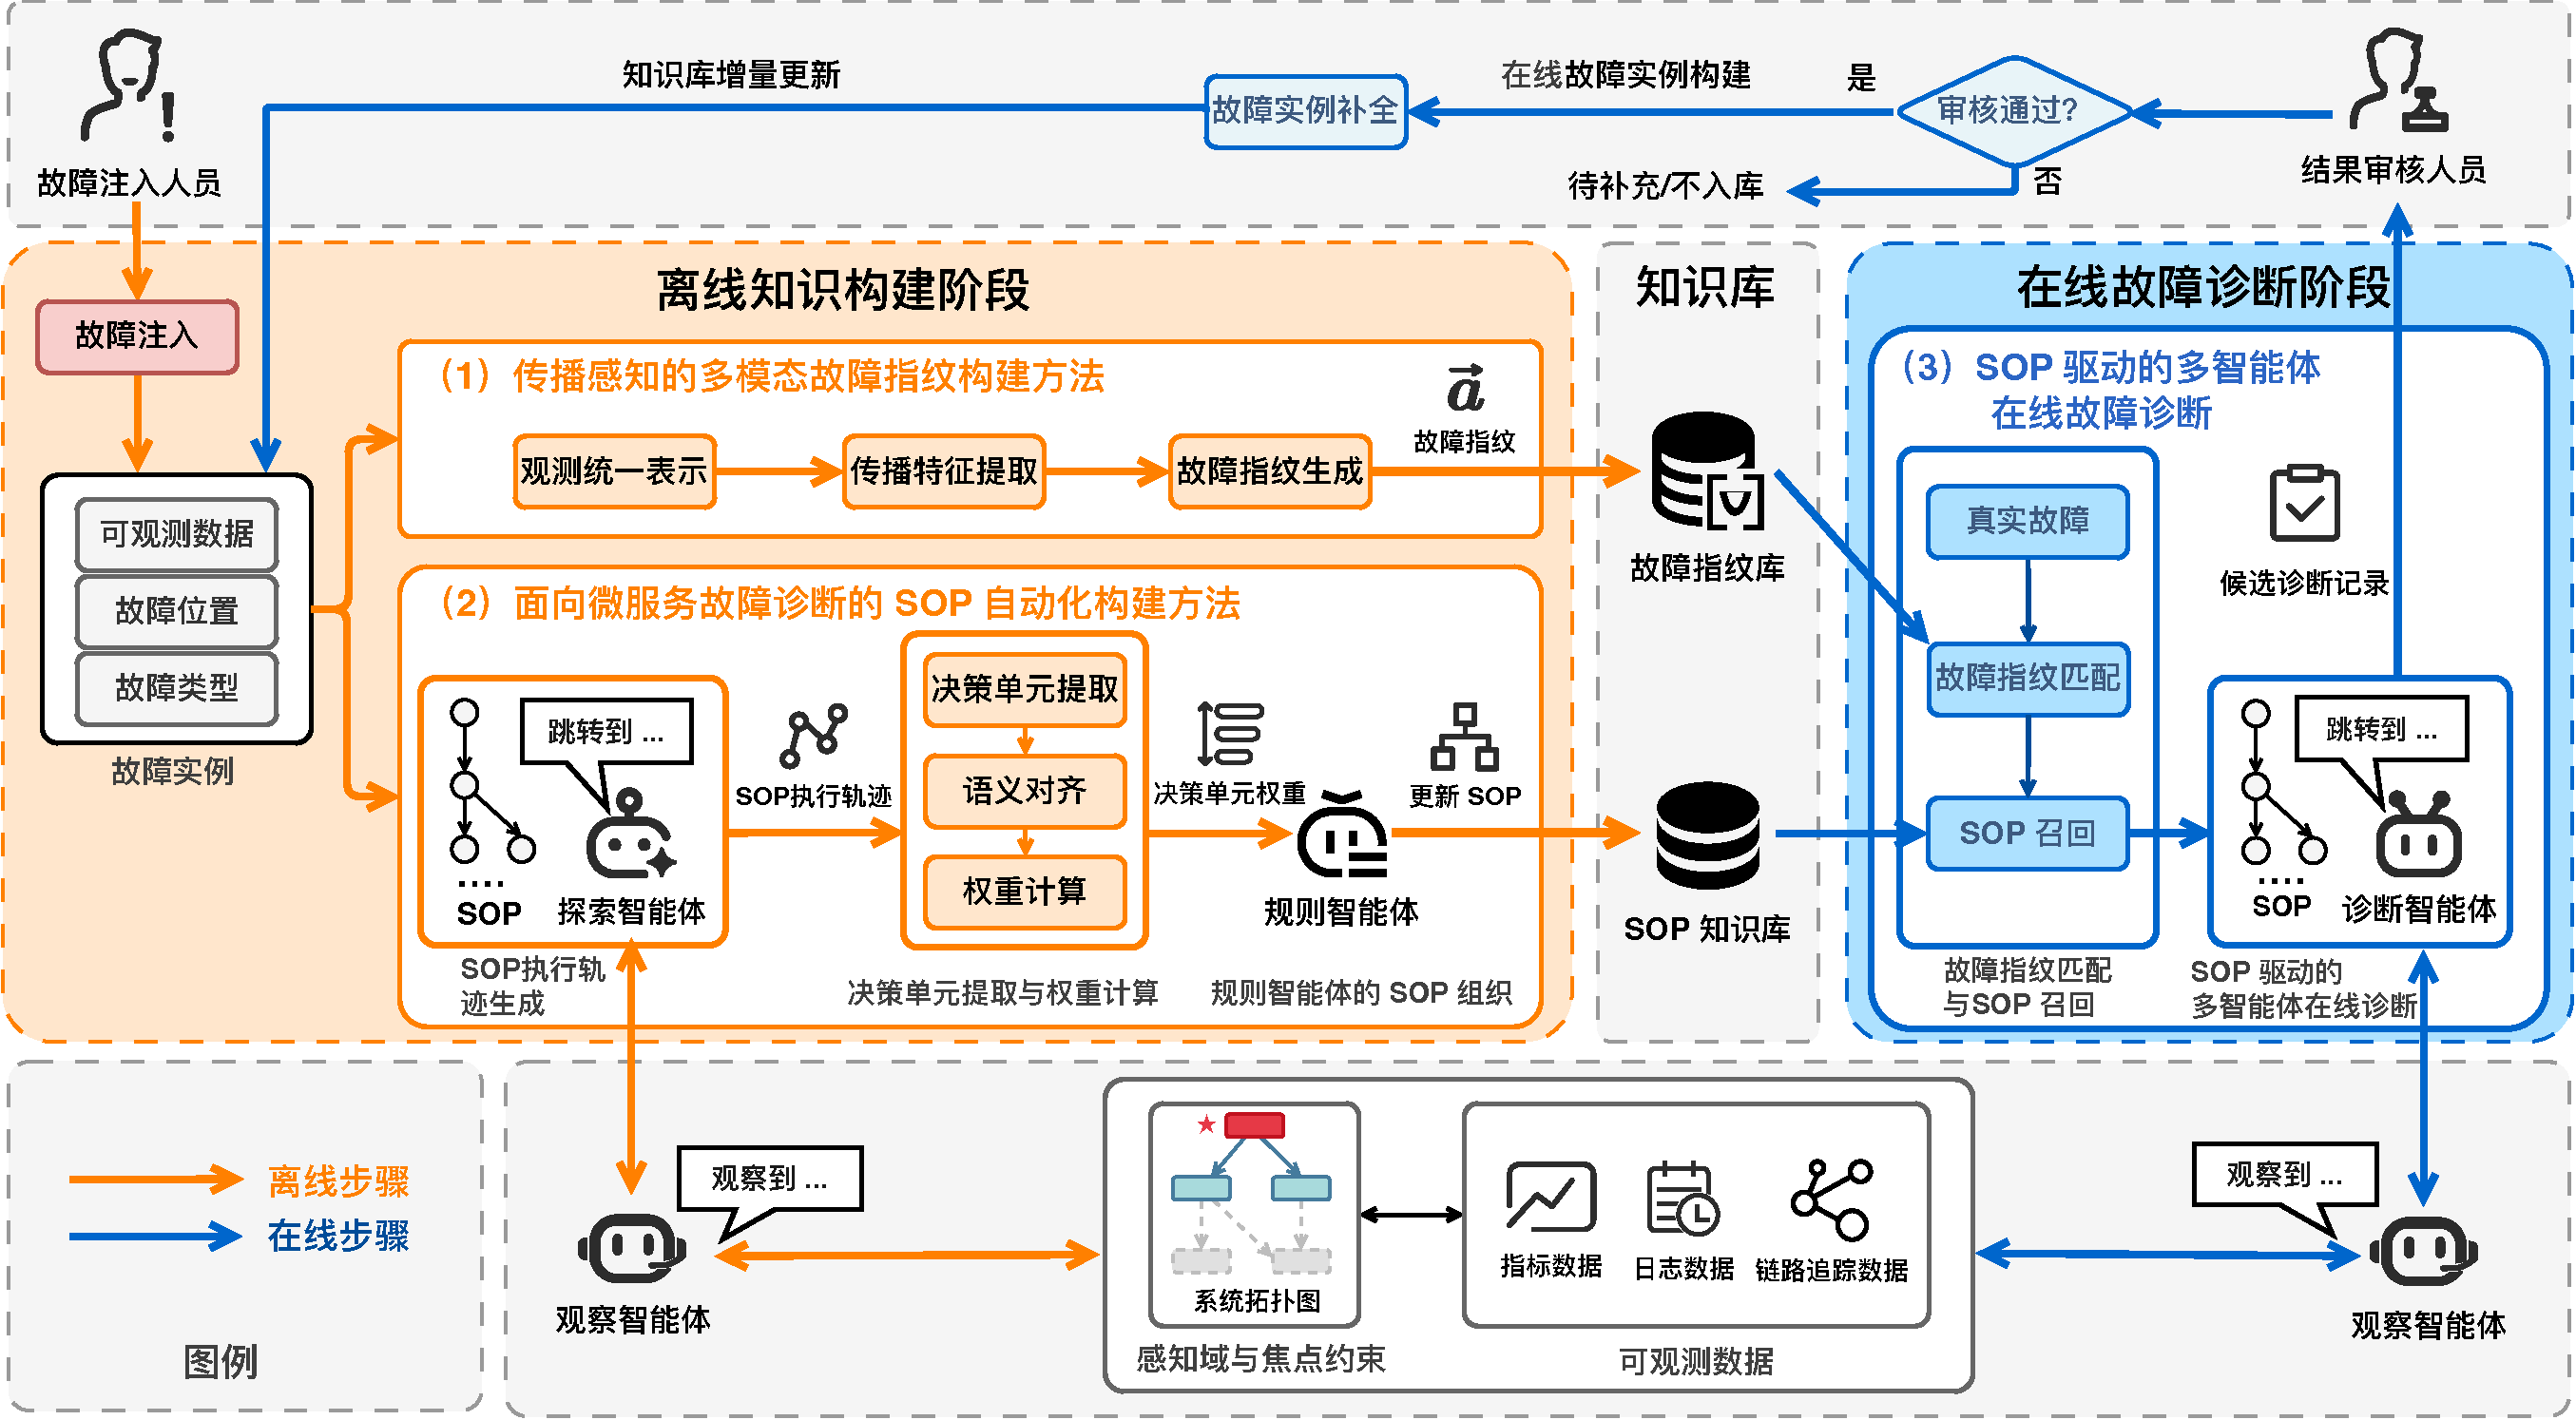
\includegraphics[width=\textwidth]{Figures-Src/Chap3-Methodology/overall-architecture/chart.pdf}
    \bicaption{经验驱动的微服务故障根因定位智能体流程}{Workflow of Experience Driven Agent-Based Root Cause Localization}
    \label{fig:overall_arch}
\end{figure}
\FloatBarrier


\textbf{离线知识构建阶段}以故障注入实验产生的有效故障实例为输入，其中包含故障窗口内的指标、日志、调用链路，以及已知的故障位置和故障类型。该阶段包含两项技术：\textbf{（1）传播感知的多模态故障指纹构建方法（第3.2节）}，用于把多模态观测数据转化为固定维度的故障指纹；\textbf{（2）面向微服务故障诊断的 SOP 自动化构建方法（第3.3节）}，用于从故障实例中生成 SOP执行轨迹、提取决策单元并组织为可执行 SOP。离线阶段完成后，系统形成故障指纹库和 SOP 知识库，分别服务于相似故障检索和在线诊断。

\textbf{在线故障诊断阶段}面向生产环境中的真实故障，对应\textbf{（3）SOP驱动的智能体在线故障诊断方法（第3.4节）}。当新故障发生时，获得当前场景观测数据生成故障指纹，检索故障指纹库中最相似的历史故障簇并召回对应 SOP。诊断智能体与观察智能体在共享观察能力支持下推进排查；若现有 SOP 无法覆盖当前分支，则进入受控逃逸模式，在有限范围内扩展路径。诊断结束后，系统生成候选诊断记录并提交人工审核。审核通过后，该记录作为新的故障实例回流离线阶段，执行故障指纹和 SOP 的增量更新。
